\section{Functional test} \label{systemtest}
Once the MPPT algorithm was working as expected, it was tested using the RT Box as the MPPT controller \cite{RTbox}. The RT Box received as analog inputs the voltage and current measured at the output of the PV simulator. The digital outputs of the RT Box were the PWM signals for switching the MOSFETs. For the tests the PV simulator \textit{E4360} from Keysight Technologies \cite{PV_simulator} is used to simulate the PV panel \textit{STP300S-24/Vd} from Suntech Power \cite{PV_panel}.  The experimental setup is shown in figure \ref{testsetup}.

At first the converter is subjected to the open-loop test. The reason for this test is to compare the measured voltages and current ripples with the calculated values from the open-loop simulation in appendix \ref{app:OL_ripple}. 
%The second test includes the thermal test. For this test the converter is tested for a longer time to identify which parts of the PCB overheated. 
Finally, a test for verifying that the P\&O algorithm was performed to see whether it behaved like in the simulation from section \ref{MPPTSimulation}. A discussion on the obtained results is carried out in section \ref{Experiment_verification}


\subsection{Open-loop test}

The open-loop test is carried out to measure the ripples in the inductor current, the input voltage and the output voltage of the converter. The test conditions were explained in section \ref{sec:componentsizing} and the graphs showing the experimental results are shown in appendix \ref{app:OL_ripple}.

The measured current ripple in the inductor is calculated from figure \ref{Openlooptestinductor} and shown in equation \ref{eq:inductor_ripple}. The minimum current is $I_{min} = 2.7A$ and the maximum current is $I_{max} = 2.98A$. The mean value for the inductor current is $\widebar{I_L}= 2.84$. 

\begin{equation} \label{eq:inductor_rippleexpirment}
\Delta I_L = \frac{I_{max}-I_{min}}{\widebar{I_L}} \cdot 100 = \frac{2.98A-2.7A}{2.84A} \cdot 100 = 9.86\%
\end{equation}

The result obtained for the output voltage ripple is shown in figure \ref{Openlooptestoutputtcapacitor}. The ripple percentage is calculated in equation \ref{eq:output_voltage_rippleexperiment} using the values obtained from the graph. 

\begin{equation} \label{eq:output_voltage_rippleexperiment}
\Delta V_{out} = \frac{V_{out,max}-V_{out,min}}{\widebar{V_{out}}} \cdot 100 = \frac{23.9082V - 23.895V }{23.9V} \cdot 100 = 0.055\%
\end{equation}

Finally, the measured input voltage ripple is shown in figure \ref{Openlooptestinputcapacitor}. It is observed from the figure that the signal is too noisy and it is not possible to identify the real voltage ripple. This is because the input voltage ripple was defined to be lower than 0.1\% and, as the input capacitor has a high capacitance, the measured ripple is neglected. \todo{check this and if it's necessary explain it better. Stef}\todo{Here it sounds like the experimental input voltage ripple is bad. We can't see it because it is so small which is a good thing}

\iffalse
\subsection{Thermal test}

For this test, the converter is supplied for 40 minutes a constant input voltage 36.9 V and input current 5.67 A. The converter is performing in buck mode with the fix duty cycles D1 = 0.96 and D2 = 0.04 in this test.The output power is in this case 250 W. The temperature of the components coil, heat sink are measured during the test because they are the critical components. Figure \ref{Testthermal} shows that 

\begin{figure}[H]
	\begin{center}
		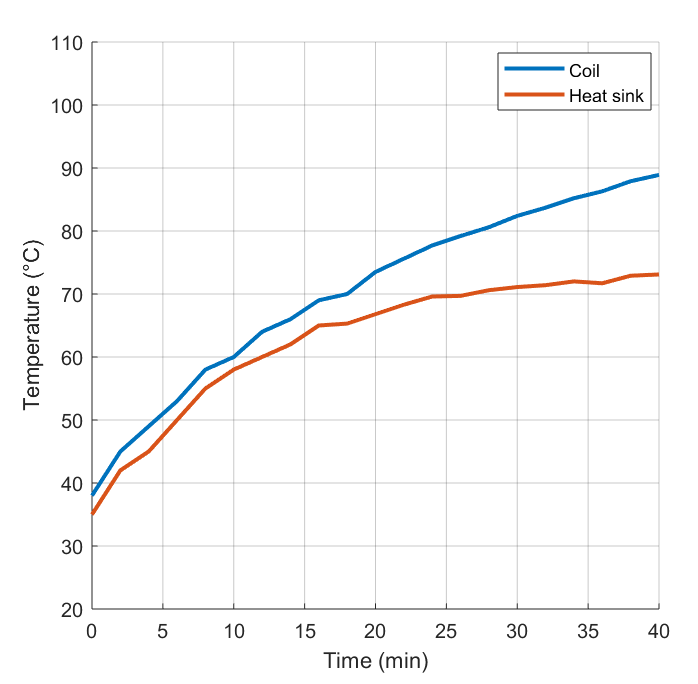
\includegraphics[width=0.65\textwidth]{../Pictures/P1/Test/Thermal_test_with_heat_sink}
		\caption{Thermal test.}
		\label{Testthermal}
	\end{center}	
\end{figure}
\fi
\subsection{MPPT test}
The MPPT test is divided into two parts, tests at STC and step change in environmental conditions. The test will be implemented for both modes of operation for the converter. For obtaining the results in buck mode a resistive load of 3$\Omega$ is used, and of 27 $\Omega$ for boost mode.

 \subsubsection*{Standard test conditions}
For the first test, the environmental conditions are set to 1000 $W /m^2$ irradiance and temperature 25 $\decC$. Figure \ref{MPPTtestbuckmode1} shows how the converter is tracking the MPP in buck mode. The left graph represents the input voltage and current of the converter. At first, the input voltage reached $V_{OC}$ as in the simulation. After 10 seconds the P\&O algorithm reaches the MPP. The average power obtained from the PV panel is 293.56 W. This can be seen in the right graph of figure \ref{MPPTtestbuckmode1}. By comparing the measured value of power with the maximum power that the PV panel can generate under these conditions, the performance of the MPPT can be quantified, this is shown in equation \ref{eq:effMPPTbuck}.

\begin{equation} \label{eq:effMPPTbuck}
\eta_{MPPT}= \dfrac{P_{PV}}{P_{MPP}} \cdot 100 = \dfrac{293.56W}{300.4W} \cdot 100 = 97.72\%  
\end{equation}


\begin{figure}[H]
	\begin{center}
		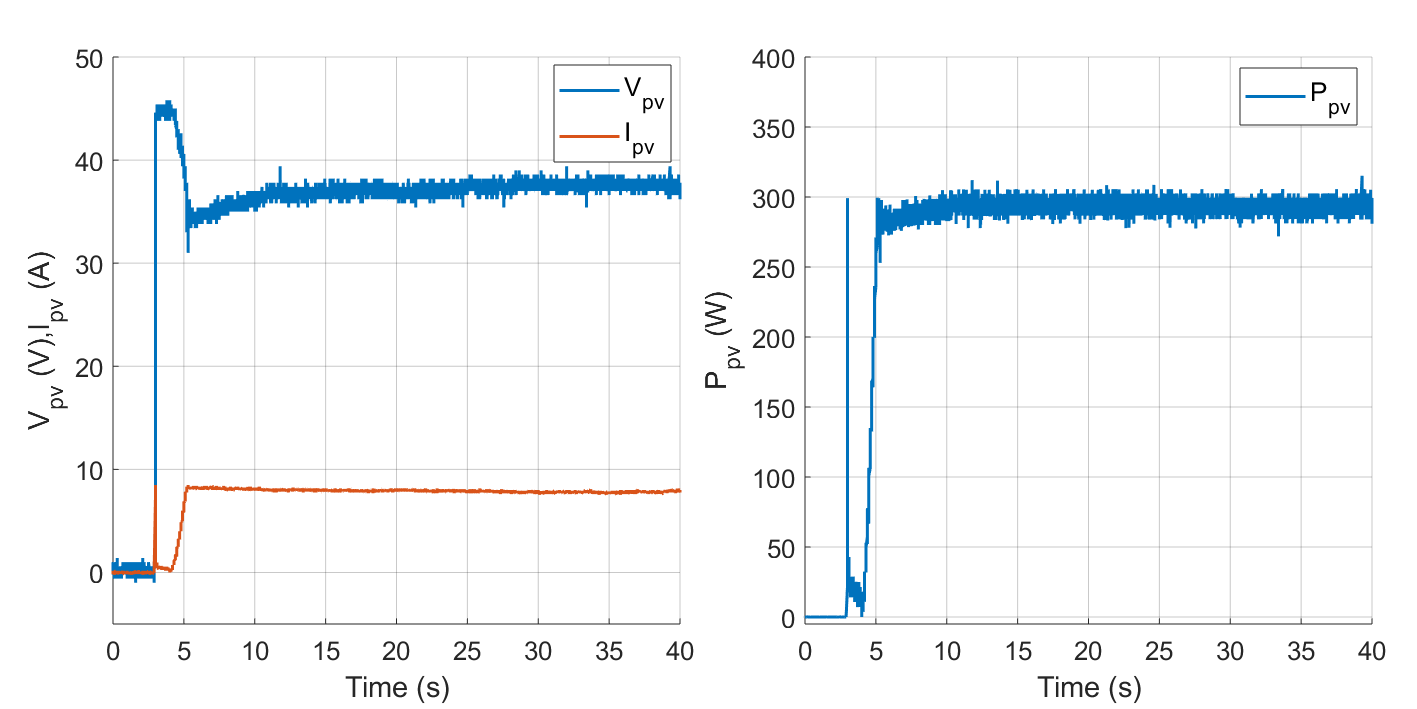
\includegraphics[width=1\textwidth]{../Pictures/P1/Test/Buck_mode_MPPT_Vin_Iin_Pin}
		\caption{Measured voltage, current and power extracted from the PV panel ($R_{L}=3\Omega$).}
		\label{MPPTtestbuckmode1}
	\end{center}	
\end{figure}

In the left graph in figure \ref{MPPTtestbuckmode2} the relationship between input and output voltage of the converter is observed. From these measurements it is possible to calculate the duty cycle in buck mode for the optimal operating point as in equation \ref{eq:measureddutybuck}. The ideal value of the duty cycle working at MPP is $D_{buck} = 0.81$.

\begin{equation} \label{eq:measureddutybuck}
D_{buck}= \dfrac{V_{out}}{V_{pv}} = \dfrac{28.29V}{37.25} = 0.7594
\end{equation}

The right graph shows the measured input and output power of the converter. From these measurements the efficiency of the converter is calculated in equation \ref{eq:effconverterbuck}, based on the average values from the graphs.

\begin{equation} \label{eq:effconverterbuck}
\eta_{converter}= \dfrac{P_{out}}{P_{pv}} \cdot 100 = \dfrac{273.44W}{293.56W} \cdot 100 = 93.15\% 
\end{equation}


\begin{figure}[H]
	\begin{center}
		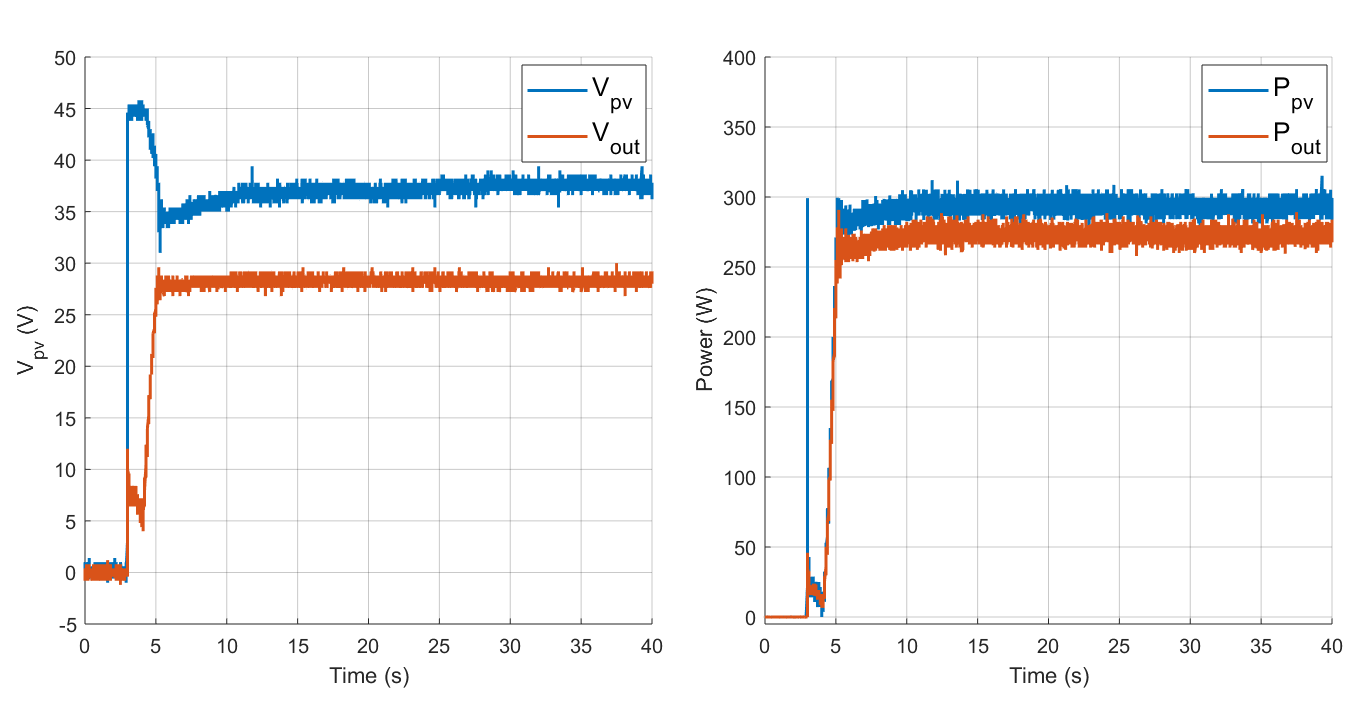
\includegraphics[width=1\textwidth]{../Pictures/P1/Test/Buck_mode_MPPT_Vin_Vout_Pin_Pout}
		\caption{Measured voltages and powers at the input and output of the converter ($R_{L}=3\Omega$).}
		\label{MPPTtestbuckmode2}
	\end{center}	
\end{figure}

Figure \ref{MPPTtestboostmode1} shows how the converter is tracking the MPP in boost mode. Here again it is observed that the MPPT is enabled after the input voltage has reached the value of open-circuit. The time the MPPT takes to reach the MPP is higher than in buck mode, reaching it in 21 seconds. By comparing the measured power with the maximum power that the PV panel can generate under STC, the MPPT's efficiency is calculated in equation \ref{eq:effMPPTboost}. It is observed that even though the system needs more time to track the MPP it does not have a significant effect in the efficiency.

\begin{equation} \label{eq:effMPPTboost}
\eta_{MPPT}= \dfrac{P_{pv}}{P_{MPP}} \cdot 100 = \dfrac{292.37W}{300.4W} \cdot 100 = 97.32\%  
\end{equation}


\begin{figure}[H]
	\begin{center}
		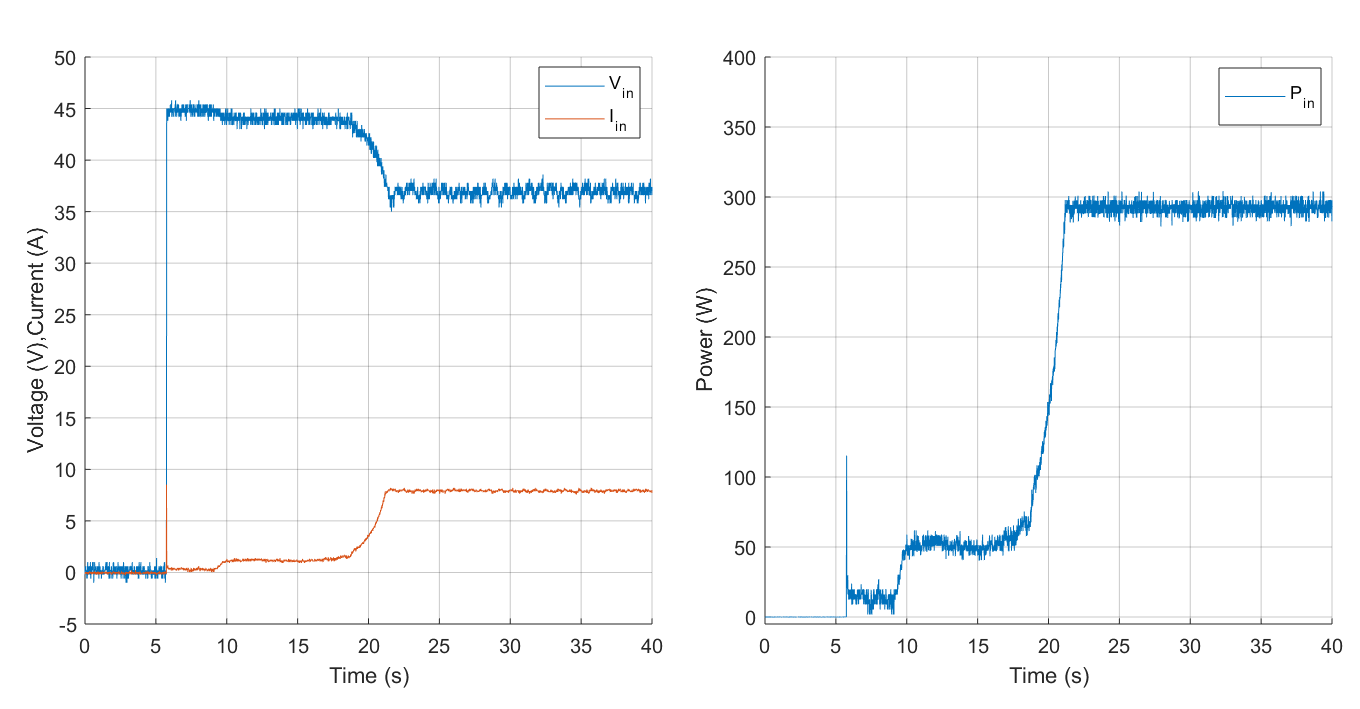
\includegraphics[width=1\textwidth]{../Pictures/P1/Test/Boost_mode_MPPT_Vin_Iin_Pin}
		\caption{Measured voltage, current and power extracted from the PV panel ($R_{L}=27\Omega$).}
		\label{MPPTtestboostmode1}
	\end{center}	
\end{figure}

%From the left graph of figure \ref{MPPTtestboostmode2} the duty cycle in boost mode for the optimal operating point can be calculated as in equation \ref{eq:measureddutyboost}. From the right graph the converter's efficiency is calculated as shown in equation \ref{eq:effconverterboost}.

%Efficiency of the converter is not considered for boost mode since the worst case happens during buck mode. The reason for this is higher currents in the components will increase the losses.

From figure \ref{MPPTtestboostmode2} the duty cycle in boost mode for the optimal operating point can be calculated as in equation \ref{eq:measureddutyboost}. The ideal value of the duty cycle to work at the MPP is 0.59.

\begin{equation} \label{eq:measureddutyboost}
D_{boost}= 1 - \dfrac{V_{pv}}{V_{out}} = 1 - \dfrac{36.93V}{88.41V} = 0.5823
\end{equation}

\iffalse
\begin{equation} \label{eq:effconverterboost}
\eta_{converter}= \dfrac{P_{out}}{P_{pv}} \cdot 100 = \dfrac{297.5W}{292.37W} \cdot 100 = 101.75\% 
\end{equation}
\fi

\begin{figure}[H]
	\begin{center}
		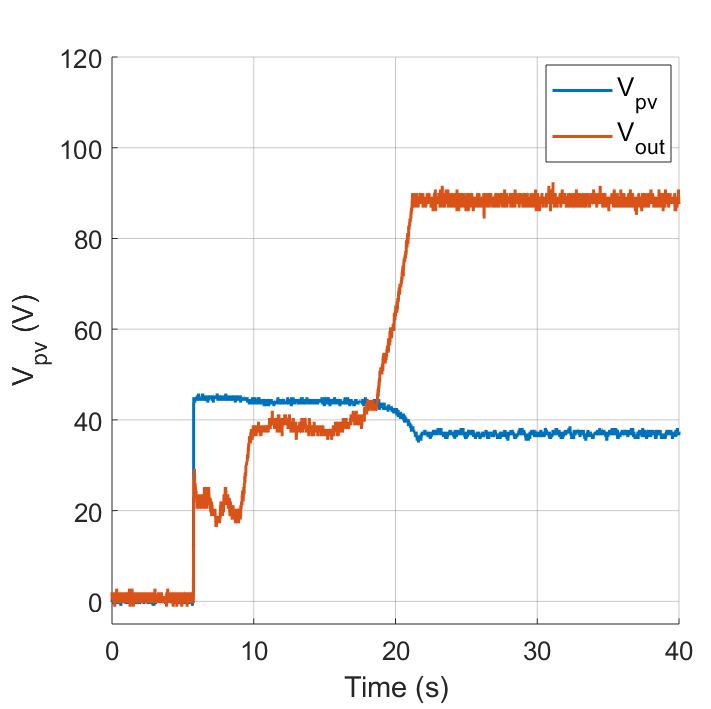
\includegraphics[width=0.6\textwidth]{../Pictures/P1/Test/Boost_mode_MPPT_Vin_Vout}
		\caption{Measured voltages at the input and output of the converter ($R_{L}=27\Omega$).}
		\label{MPPTtestboostmode2}
	\end{center}	
\end{figure}


\iffalse
\begin{figure}[H]
	\begin{center}
		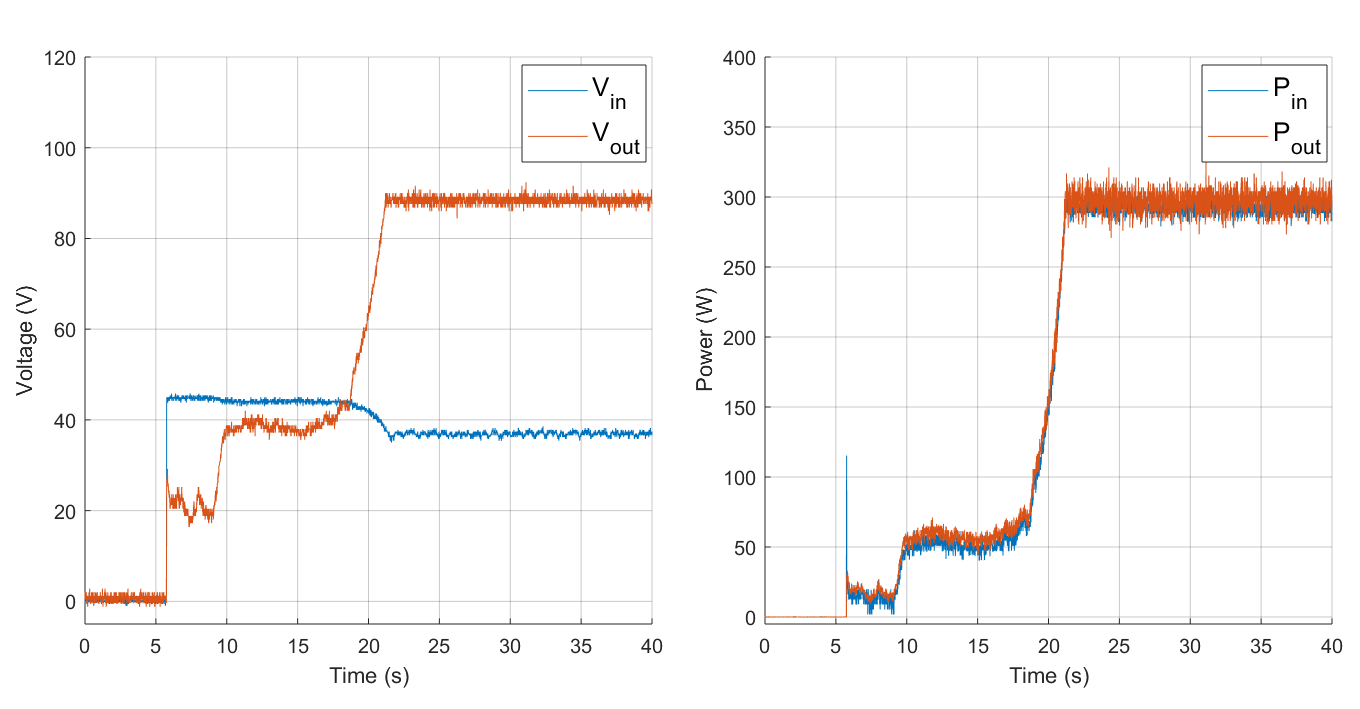
\includegraphics[width=1\textwidth]{../Pictures/P1/Test/Boost_mode_MPPT_Vin_Vout_Iin_Pin_Pout}
		\caption{Measured voltages and powers at the input and output of the converter ($R_{L}=27\Omega$).}
		%\label{MPPTtestboostmode2}
	\end{center}	
\end{figure}
\fi


\subsubsection*{Change in irradiance and temperature}

For this test the converter was set to work in buck mode by fixing a resistive load of 3$\Omega$. Figure \ref{MPPTtestbuckmodeir} shows the measurements obtained for voltage, current and power generated by the PV simulator. It is observed that the MPPT detects the change in irradiance and tracks the MPP. The MPPT's efficiency changes from 95.96\% to 93.78\% when a sudden change in irradiance from 1000-800$W/m^2$ is detected. The time response is 6.6 seconds.

\begin{figure}[H]
	\begin{center}
		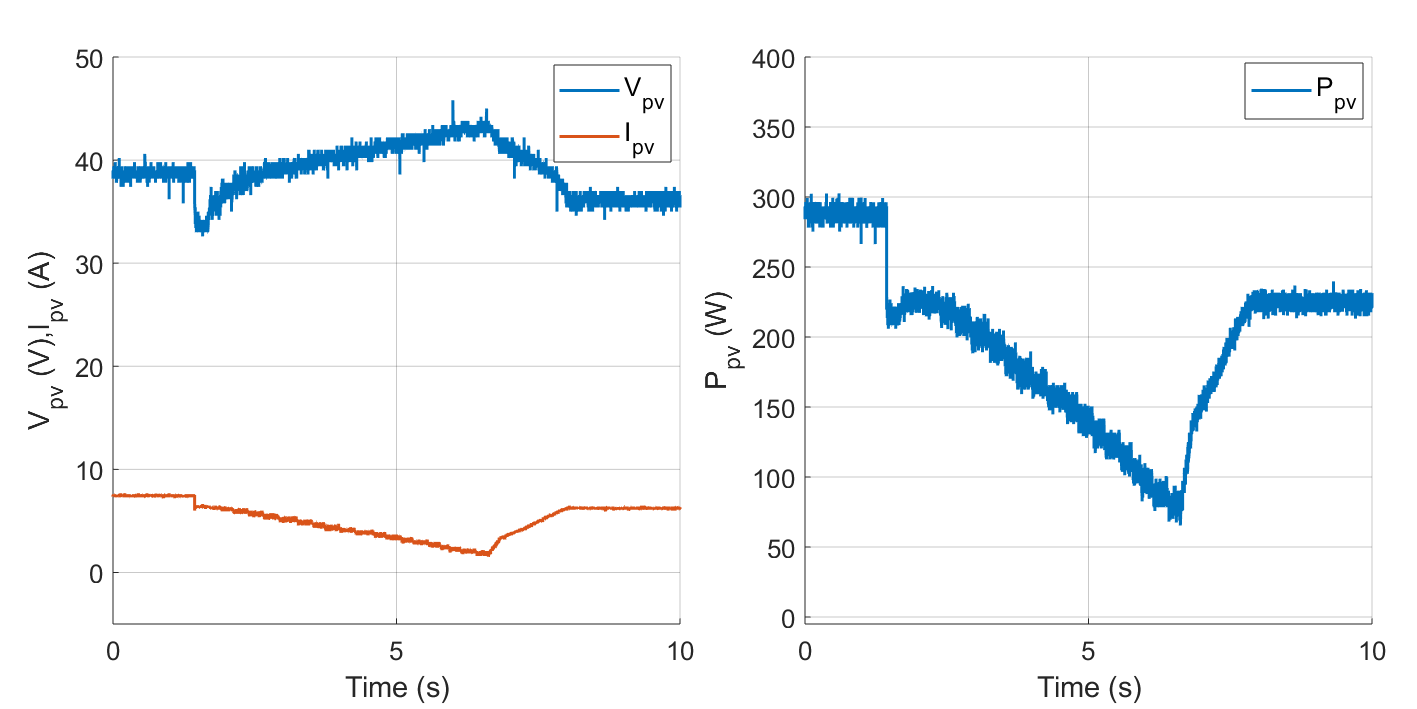
\includegraphics[width=1\textwidth]{../Pictures/P1/Test/Buck_mode_MPPT_Vin_Iin_Pin_irriadance_change}
		\caption{Measured voltage,current and powers at the input of the converter with a change in irradiance from 1000$W/m^2$ to 800$W/m^2$ ($R_{L}=3\Omega$).}
		\label{MPPTtestbuckmodeir}
	\end{center}	
\end{figure}

Figure \ref{MPPTtestbuckmodet} shows the results obtained for a sudden change in temperature from 25$\decC$ to 15$\decC$. It is observed that the generated power increases with decreasing temperature. The MPPT's efficiency improves in this case comparing with the variation in irradiance. It changes from 99.2\% to 98.4\% in 4.1 seconds. 

\begin{figure}[H]
	\begin{center}
		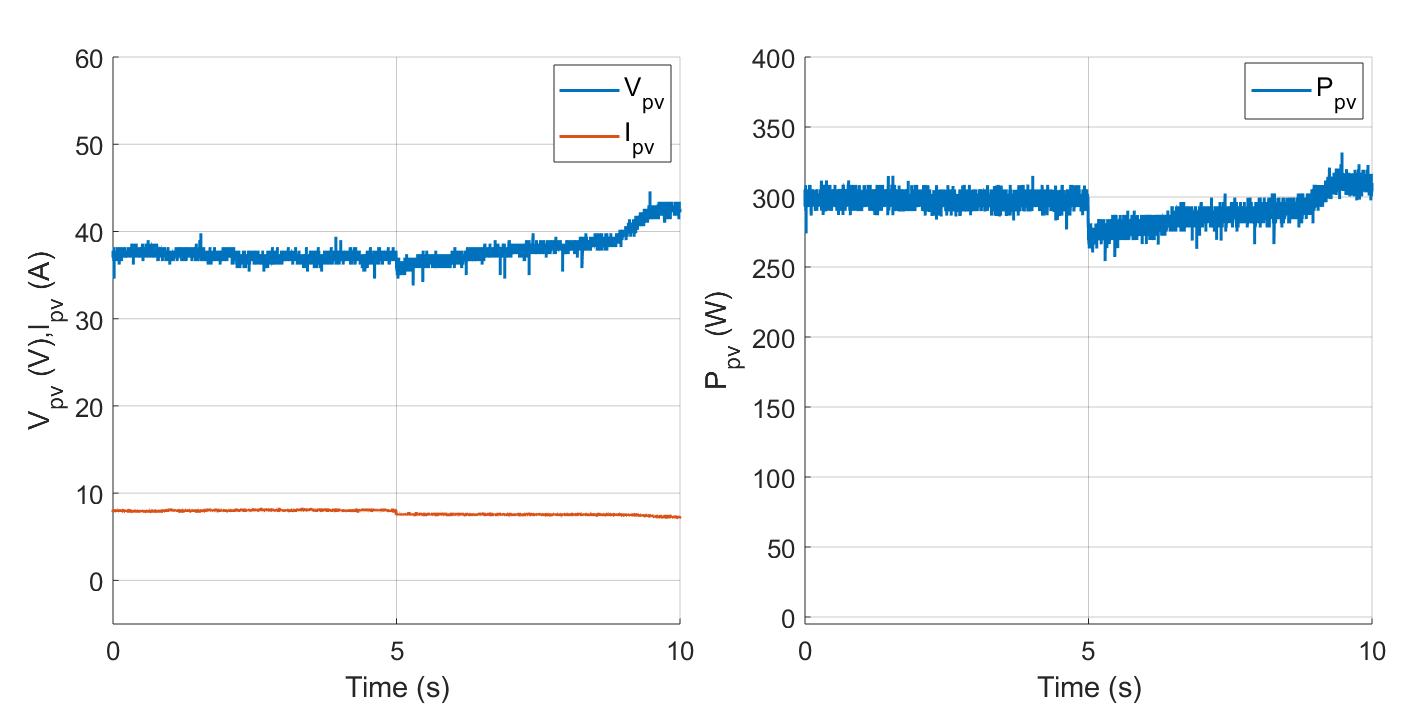
\includegraphics[width=1\textwidth]{../Pictures/P1/Test/Buck_mode_MPPT_Vin_Iin_Pin_temperature_change}
		\caption{Measured voltage,current and power at the input of the converter with a change in temperature from 25$\decC$ to 15$\decC$ ($R_{L}=3\Omega$).}
		\label{MPPTtestbuckmodet}
	\end{center}	
\end{figure}